\chapter{求函数从$a$到$b$的和与积分}
函数有两个基本性质——变率与和,在前一章,我们研究了函数的瞬时变率的概念,即
\[f'(x_0) =\lim_{h\to 0} \frac{f (x_0+h) -f (x_0)}{h}\]
以及它的应用,在本章我们将研究对于一个给定函数$f(x)$“求从$a$到$b$的和”这个概念。在给出定义之前,我们先举几个实例来看一看。

\paragraph{速率与距离} 
一列行驶中的火车,它的行进速率$v$是时间$t$的函数,即
$v=f(t)$, 如图3.1, 我们可以从速率表读得当时的速率,很自然地,我们想知道火车在从$t=a$到$t=b$这一段时间间隔内一共走了多少路程。从函数的观点看,所谓求在时间$[a,b]$内所走过的距离就是求速率函数$v=f(t)$由$t=a$到$t=b$的和。

\begin{figure}[htp]
    \centering
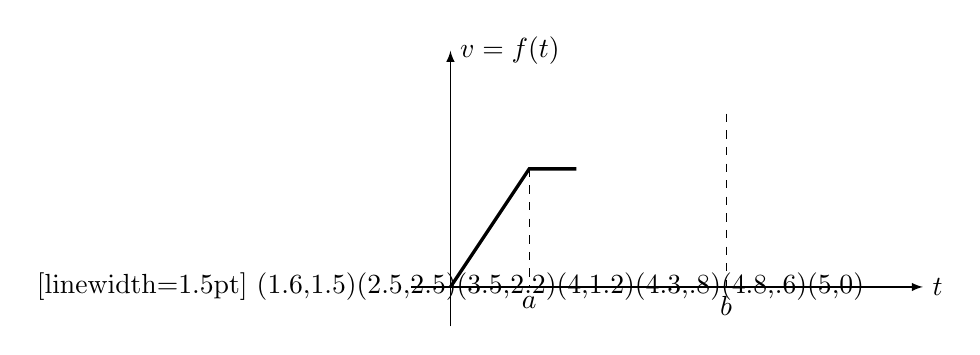
\begin{tikzpicture}[>=latex]
\draw[->](-.5,0)--(6,0)node[right]{$t$};
\draw[->](0,-.5)--(0,3)node[right]{$v=f(t)$};
\draw[very thick](0,0)--(1,1.5)--(1.6,1.5);
\draw[dashed](1,1.5)--(1,0)node[below]{$a$};
\node at (0,0){
\pscurve[linewidth=1.5pt] (1.6,1.5)(2.5,2.5)(3.5,2.2)(4,1.2)(4.3,.8)(4.8,.6)(5,0)
};
\draw[dashed](3.5,2.2)--(3.5,0)node[below]{$b$};

\end{tikzpicture}
    \caption{}
\end{figure}

让我们用$D(f,[a,b])$
表示所走过的距离,这个记号强调$D$依赖于$f$和区间$[a,b]$。

\paragraph{变力所作的功}

假定某物体在一个平行于$OX$轴的力$P$的作 用下沿直线
$OX$运动,力$P$的方向与物体运动的方向一致,并且力的大小随离开$O$点的距离而改变,即变力$P$是所在点的横坐标$x$的函数$P=P(x)$, 如图3.2。假定物体在这个变力$P$作用之下,从直线$OX$的一点$a$移到另一点$P$, 那么力$P$所作的功就是变力函数$P(x)$由$x=a$到$x=b$的和,我们用
$W (P, [a,b])$
表示力$P$所作的功,它表明$W$依赖于$P(x)$和$[a,b]$。

\begin{figure}[htp]
    \centering
    \begin{minipage}[t]{0.48\textwidth}
    \centering
    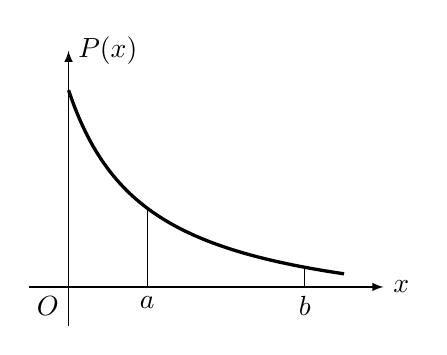
\begin{tikzpicture}[>=latex, scale=1]
\draw[->](-.5,0)--(4,0)node[right]{$x$};
\draw[->](0,-.5)--(0,3)node[right]{$P(x)$};
\draw[domain=0:3.5, samples=100, very thick]plot(\x, {3/(\x+1)-.5});
\draw(1,0)node[below]{$a$}--(1,1);
\draw(3,0)node[below]{$b$}--(3,.25);
\node at (0,0)[below left]{$O$};
    \end{tikzpicture}
    \caption{}
    \end{minipage}
    \begin{minipage}[t]{0.48\textwidth}
    \centering
    \begin{tikzpicture}[>=latex, scale=1]
\draw[->](-.5,0)--(4,0)node[right]{$x$};
\draw[->](0,-.5)--(0,3)node[right]{$y$};
\draw[domain=0:3.5, samples=100, very thick]plot(\x, {.3*(\x-2.2)^2+.5})node[above right]{$y=f(x)$};
\node at (0,0)[below left]{$O$};
\draw(.5,0)node[below]{$a$}--(.5,1.367)node[above right]{$M_0$};
\draw(3,0)node[below]{$b$}--(3,.692)node[above]{$M$};
\fill[pattern=north east lines, domain=.5:3, samples=100, very thick]plot(\x, {.3*(\x-2.2)^2+.5})--(3,.692)--(3,0)--(.5,0)--(.5,1.367);


    \end{tikzpicture}
    \caption{}
    \end{minipage}
\end{figure}

\paragraph{曲边梯形的面积}

令$y=f(x)$是函数$f$的图象,表示一条曲线,如图3.3. 我们要求曲线上的一段弧$M_0M$ 与其两端的纵坐标线及$x$轴上的线段$[a,b]$所围成的图形的面积。这样的图形(它有三条边是直线,其中两条互相平行,第三条与前两条
互相垂直,而第四条边是曲线)叫做曲边梯形。显然曲边梯形的面积$A$依赖于$y=f(x)$和$x$轴上的线段$[a,b]$, 记这一面积为$A (f, [a,b])$。

在上一章,我们利用函数$f(x)$和它的图象之间的对应关系,就可以把函数的变率和它的图象的切线的斜率相对应地一并分析讨论,这样,一方面可以把函数的变率这种“数量”的概念用切线来形象化,便于想象;而另一方面又可以把“切线”这种几何概念数量化,便于计算,在这一章,我们也要利用函数$f(x)$和它的图象之间的对应关系,把函数$f(x)$由$x=a$到$x=b$的“和”与曲线$y=f(x)$的曲边梯形的“面积”相对应地一并分析讨论,并且说明函数的“求从$a$到$b$的和”恰好对应于求曲边梯形的面积。这也就是为什么把函数“求从$a$到$b$的和”这种基本运算叫做积分的道理。

\section{“和”与“面积”}
对于任意曲线围成的图形,我们还没有规定它的“面积”的意义,和它密切相关的“函数从$a$到$b$的和”的概念至今也没有明确的解析的定义。在这一节我们要把这两个概念由“直观的定性理解”推进到“数量化的定量定义”。唯有确立了它们的“解析的定义”,它们才真正地成为能算好用的量。

\subsection{“和”与“面积”的基本性质}
现在让我们先从“函数的和”与“曲线形的面积”的直观内涵来分析一下它们分别所应有的基本性质。

\subsubsection{“曲线形的面积”的基本性质}

从面积的直观内涵容易看出下列两点:
\begin{enumerate}
\item (单调性)设区域$R_1$包含在$R_2$之内,即$R_1\subseteq R_2$, 则:
$R_1$的面积$\le R_2$的面积.(图3.4)
\item (可加性)设区域$R$可以用一条曲线分割成两块区
域$R_1+R_2$, 则有:
$R$的面积$=R_1$的面积$+R_2$的面积.(图3.5)
\end{enumerate}

\begin{figure}[htp]
    \centering
    \begin{minipage}[t]{0.48\textwidth}
    \centering
    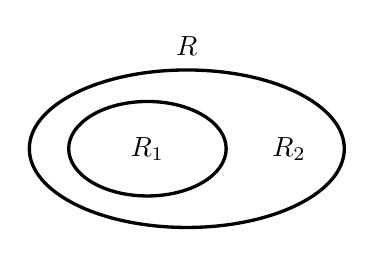
\begin{tikzpicture}[>=latex, scale=1]
\draw[very thick](0,0) ellipse [x radius=2, y radius =1];
\draw[very thick](-.5,0) ellipse [x radius=1, y radius =.6];
\node at (0,1.3){$R$};
\node at (-.5,0){$R_1$};
\node at (1.3,0){$R_2$};
    \end{tikzpicture}
    \caption{}
    \end{minipage}
    \begin{minipage}[t]{0.48\textwidth}
    \centering
    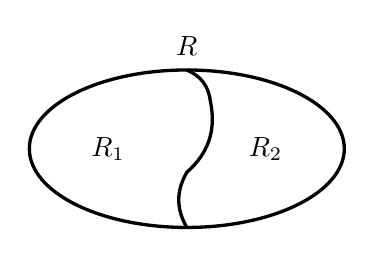
\begin{tikzpicture}[>=latex, scale=1]
\draw[very thick](0,0) ellipse [x radius=2, y radius =1];
\node at (0,1.3){$R$};
\node at (-1,0){$R_1$};
\node at (1,0){$R_2$};
\draw[very thick](0,1) to [bend left](.3,.6)to [bend left](0,-.3)to [bend right](0,-1);
    \end{tikzpicture}
    \caption{}
    \end{minipage}
\end{figure}

\subsubsection{“函数的和”的基本性质}

同样地,从“函数从$a$到$b$的和”的直观内涵容易看出下列两个基本性质,即

\begin{blk}{性质1:单调性}
设函数$f(t)$和$g(t)$在$a\le t\le b$上,$f(t)\le g(t)$恒成立,那么:

“$f(t)$由$t=a$到$t=b$的和”$\le $“$g(t)$由$t=a$到$t=b$
的和”。
\end{blk}

例如,两部车子在$t=a$到$t=b$的时间内,甲车的速率$f(t)\le $乙车的速率$g(t)$, 则甲车在上述时间内所经过的里程$\le $乙车在上述时间内所经过的里程。

\begin{blk}{性质2:可加性}
设$a<b<c$,那么,有:

“$f(t)$由$t=a$到$t=b$的和”$+$“$f(t)$由$t=b$到$t=c$的和”$=$“$f(t)$由$t=a$到$t=c$的和”。
\end{blk}

上述基本性质是一目了然的,让我们先用来说明一些简单的基本事实。

\begin{example}
    设函数$y=f(t)=k$(常数),则由和的直观内涵,显然应有:
\[\text{常数函数从$a$到$b$的和}=k(b-a)\]

例如,以等速率每小时$k$公里行驶的火车从$t=a$小时到$t=b$小时内所走的总里程应该是$k(b-a)$公里。

现在让我们利用函数的图象来观察上述数值$k(b-a)$的几何意义。

\begin{figure}[htp]
    \centering
    \begin{minipage}[t]{0.48\textwidth}
    \centering
    \begin{tikzpicture}[>=latex, scale=.9]
\draw[->](-.5,0)--(5,0)node[right]{$t$};
\draw[->](0,-.5)--(0,3)node[right]{$y$};
\fill[pattern=north east lines](1,0) rectangle (4,1.5);
\draw[dashed](0,1.5)--(1,1.5)--(1,0)node[below]{$t=a$};
\draw[dashed](4,1.5)--(4,0)node[below]{$t=b$};
\node at (0,0)[below left]{$O$};
\draw[very thick](1,1.5)--(4,1.5);
\node at (0,.75)[left]{$k>0$};
\node at (2.5,.75){\Large $+$};

    \end{tikzpicture}
    \caption{}
    \end{minipage}
    \begin{minipage}[t]{0.48\textwidth}
    \centering
    \begin{tikzpicture}[>=latex, scale=.9]
\draw[->](-.5,0)--(5,0)node[right]{$t$};
\draw[->](0,-2)--(0,1.5)node[right]{$y$};
\fill[pattern=north east lines](1,0) rectangle (4,-1.5);
\draw[dashed](0,-1.5)--(1,-1.5)--(1,0)node[above]{$t=a$};
\draw[dashed](4,-1.5)--(4,0)node[above]{$t=b$};
\node at (0,0)[below left]{$O$};
\draw[very thick](1,-1.5)--(4,-1.5);
\node at (0,-.9)[left]{$k<0$};
\node at (2.5,-.75){\Large $-$};
    \end{tikzpicture}
    \caption{}
    \end{minipage}
\end{figure}

\begin{enumerate}
    \item 当$k>0$时,函数$f(t)=k$的图象在$t$轴上方,$k(b-a)$对应于一个矩形的面积,如图3.6中阴影部分的面积.
    \item 当$k<0$时,函数$f(t)=k$的图象在$t$轴下方,$k(b-a)$对应于一个矩形的面积的负值,如图3.7中阴影部分的面积的负值。
\end{enumerate}

假如我们把$t$轴之上的面积定义为正的,而把$t$轴之下的面积定义为负的,则当$y=k$(常数)时,常数函数从$a$到$b$的和$=k(b-a)=$上述的有号面积。
\end{example}

\begin{example}
设$y=f(t)$是一个阶梯函数,即分段地是常数函数:
\[0=t_0<t_1<t_2<\cdots<t_{i-1}<t_i<\cdots <t_n=b\]
当$t_{i-1}\le t<t_i$时,$f(t)=k_i,\; i=1,2,\ldots,n$。由性质2,我们可以分段地用常数函数求和,就可以得到阶梯函数$f(t)$从$a$到$b$的和:
\[k_1 (t_1-t_0) +k_2 (t_2-t_1) +\cdots +k_n (t_n-t_{n-1})\]

作出阶梯函数的图象(图3.8),上述函数和就等于下列逐段由矩形并起来的区域的“有号面积”。
\begin{figure}[htp]
    \centering
\begin{tikzpicture}[>=latex, yscale=.7]
\draw[->](-5,0)--(7,0)node[right]{$t$};
\draw[->](0,-2)--(0,4)node[right]{$y=f(t)$};
\node at (0,0)[above right]{$O$};

\foreach \x/\xtext in {-3/t_1, -1/t_2, 1.5/t_3, 2.5/t_4, 3.5/t_5, 4.3/t_6, 5.5/t_{n-1},-4.5/{t_0=a},6.5/{t_n=b}}
{
    \node at (\x,0)[below]{$\xtext$};
}

\draw[pattern=north east lines, thick](-4.5,0) rectangle(-3,1.5);
\draw[pattern=north east lines, thick](-3,1) rectangle(-1,0);
\draw[pattern=north east lines, thick](-1,0) rectangle(1.5,-1.5);
\draw[pattern=north east lines, thick](1.5,0) rectangle(2.5,1);
\draw[pattern=north east lines, thick](2.5,0) rectangle(3.5,2);
\draw[pattern=north east lines, thick](3.5,0) rectangle(4.3,-1);
\draw[pattern=north east lines, thick](5.5,0) rectangle(6.5,1);
\foreach \x in {-3.75, -2, 2, 3, 6}
{
    \node at (\x,.5){$+$};
}
\foreach \x in {.75, 3.9}
{
    \node at (\x,-.5){$-$};
}
\node at (4.8,.5){…};\node at (4.8,-.5){…};

\end{tikzpicture}
    \caption{}
\end{figure}
\end{example}

\subsection{逼近法求和}

对于一个比较一般的函数,例如$y=kt+c$, $y=t^2$, $y=\sin t$等等,我们必须给函数的和下一个适当的定义,同时要提供计算这个和的方法,这里我们将要再一次地用逼近法的观点去解答上述问题,回顾上一章讨论变率时,我们的基本想法是用折线函数去逼近一般的平滑函数,所以折线函数是讨论函数变率的简单好用的基本函数,因为它们的变率十分简单,分段地是个常数而且无限逼近函数在某一点的变率,由上一段的讨论;我们知道阶梯函数的“从$a$到$b$的和”是十分简明的,它们在“函数求从$a$到$b$的和”这方面是不是也扮演着
这种既简单又基本的角色呢?这就得看一看能否用阶梯函数的从$a$到$b$的和去无限逼近一般性的“函数从$a$到$b$的和”了。

现在让我们使用几个简单的实例来试试看。

\begin{example}
假设物体以初速度$u$, 加速度$a>0$在直线上运动,于是物体在任何时刻$t$的速度是$v=f (t) =u+at$, 求物体从$t=0$到$t=T$时所经过的距离,即求速度函数$f(t)$在时间间隔$[0,T]$上的和.
\end{example}

\begin{analyze}
    一个自然的作法是用两个阶梯函数$g_n(t)$和$G_n(t)$把上述函数$f(t)=u+at$夹逼在中间,即
    \[g_n(t)\le f(t)\le G_n(t)\]
对于任何$0\le t\le T$都成立,那么由性质1,$g_n(t)$从0到$t$的和$\le f(t)$从$0$到$T$的和$\le G_n(t)$从0到$T$的和。

如果能使$g_n(t)$从0到$T$的和与$G_n(t)$从0到$T$的和,当$n\to\infty$时的极限相同,则由上述夹逼关系就可以看出$f(t)$从0到$T$的和必须等于这个共同极限.
\end{analyze}

\begin{figure}[htp]
    \centering
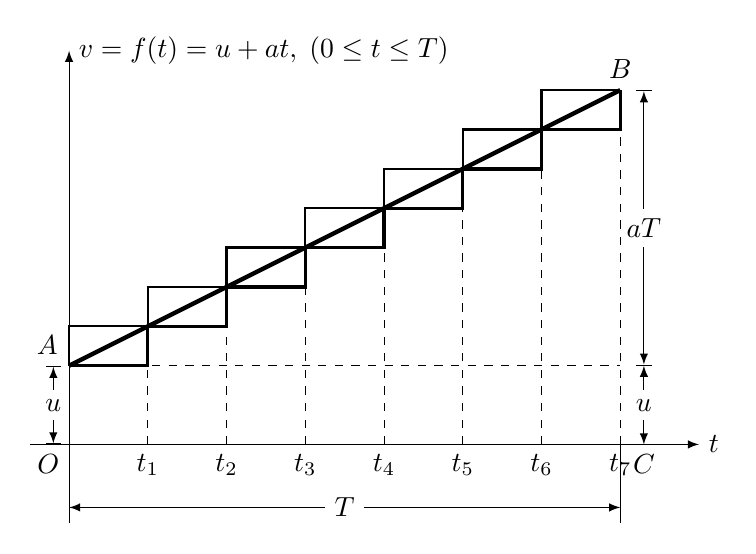
\begin{tikzpicture}[>=latex]
\draw[->](-.5,1)--(8,1)node[right]{$t$};
\draw[|<->|](-.2,1)--node[fill=white]{$u$}(-.2,2);
\draw[->](0,0)--(0,6)node[right]{$v=f(t)=u+at,\; (0\le t\le T)$};
\node at (0,1)[below left]{$O$};
\draw[ultra thick](0,2)node[above left]{$A$}--(7,5.5)node[above]{$B$};
\draw[<->](7.3,1)node[below]{$C$}--node[fill=white]{$u$}(7.3,2);
\draw[|<->|](7.3,5.5)--node[fill=white]{$aT$}(7.3,2);
\foreach \x in {1,2,3,...,6,7}
{
    \draw[dashed](\x,1)node[below]{$t_{\x}$}--(\x,2+\x*.5);
    \draw[very thick](\x-1, 1.5+\x*0.5)--(\x, 1.5+ \x*0.5)--(\x, 2+\x*0.5);
    \draw[thick](\x-1, 1.5+\x*0.5)--(\x-1, 2+\x*0.5)--(\x, 2+ \x*0.5);
}
\draw[dashed](0,2)--(7,2);
\draw(7,0)--(7,1);
\draw[<->](0,.2)--node[fill=white]{$T$}(7,.2);
\end{tikzpicture}
    \caption{}
\end{figure}

下面就是把上述想法付诸实践的具体做法之一。

\begin{solution}
\begin{enumerate}
    \item 把时间间隔$n$等分,取分点$t_i=\frac{i}{n}T,\; i=0,1, 2,\ldots,n$, 于是在每个分点$t_i=\frac{i}{n}T$处的速度分别是
\[f (t_0) =f (0) =u,\;  f(t_1) =u+at_1,\; f (t_3) =u+at_2,\ldots,f (t_n) =f (T) =u+aT\]
\item 用阶梯函数近似代替$v=f(t)=u+at$. 

假设物体在时间的每个小区间$[t_i,t_{i+1}],\; i=0,1, 2,\ldots,(n-1)$内,以小区间起点处的速度作匀速运动,我们得到一个速度的阶梯函数
\[g_n (t)=f(t_i)=u+at_i,\quad t_i\le t<t_{i+1},\quad i=0,1,2,\ldots,(n-1)\]
因为$f(t)=u+at$是严格递增的,所以$g_n(t)$有以下性质:
\[g_n (t)=f(t_i)\le f(t),\quad t_i\le t<t_{i+1},\quad i=0,1,2,\ldots,(n-1)\]
从而,对于任何$0\le t\le T$,有$g_n(t)\le f(t)$.

假设物体在时间的每个小区间$[t,t+1],\; i=0,1, 2,\ldots,(n-1)$内,以小区间终点处的速度作匀速运动,我们得到另一个速度的阶梯函数
\[G_n(t)=f(t_{i+1})=u+at_{i+1},\quad t_i< t\le t_{i+1},\quad i=0,1,2,\ldots,(n-1)\]

由于$f(t)=u+at$是递增的,所以$G(t)$有以下性质
\[G_n (t)=f(t_{i+1})\ge f(t),\quad t_i< t\le t_{i+1},\quad i=0,1,2,\ldots,(n-1)\]
从而对于任何$0\le t\le T$,有
\[G_n(t)\ge f(t)\]
这样,我们就得到了$v=f(t)$的夹逼阶梯函数:
\[ g_n(t) \le f (t) \le G_n (t),\quad 0\le t\le T\]

(在图3.8中,绘出了$f(t)=u+at$的图象和当$n=7$时阶梯函数$g_7(t)$和$G_7(t)$的图象.)

\item 求阶梯函数的总和

应用基本性质2, 我们得到$g_n(t)$从0到$T$的和
\[f(t_0)(t_1-t_0)+f(t_1)(t_2-t_1)+\cdots+f (t_{n-1}) (t_n-t_{n-1})\]

$\because\quad t_1-t_0=t_2-t_1=\cdots=t_n-t_{n-1}=\frac{T}{n}$

因此:
\[\begin{split}
\text{$g_n(t)$从0到$T$的和}&=\left[f(t_0)+f(t_1)+\cdots+f(t_{n-1})\right]\cdot \frac{T}{n}\\
&=\left[u+(u+at_1)+(u+at_2)+\cdots +(u+at_{n-1})\right]\cdot \frac{T}{n}\\
&=\left[nu+a(t_1+t_2+\cdots+t_{n-1})\right]\cdot \frac{T}{n}\\
&=\left[nu+a\left(\frac{T}{n}+\frac{2T}{n}+\cdots+\frac{(n-1)T}{n}\right)\right]\cdot \frac{T}{n}\\
&=uT+a\cdot [1+2+\cdots+(n-1)]\left(\frac{T}{n}\right)^2\\
&=uT+a\cdot \frac{n(n-1)}{2}\cdot \frac{T^2}{n^2}\\
&=uT+\frac{1}{2}aT^2\left(1-\frac{1}{n}\right)
\end{split}\]

\[\begin{split}
    \text{$G_n(t)$从0到$T$的和}&=f(t_1)(t_1-t_0)+f(t_2)(t_2-t_1)+\cdots+f(t_n)(t_n-t_{n-1})  \\
   &= \left[f(t_1)+f(t_2)+\cdots+f(t_{n})\right]\cdot \frac{T}{n}\\
    &=\left[(u+at_1)+(u+at_2)+\cdots +(u+at_{n})\right]\cdot \frac{T}{n}\\
    &=\left[nu+a\left(\frac{T}{n}+\frac{2T}{n}+\cdots+\frac{nT}{n}\right)\right]\cdot \frac{T}{n}\\
    &=uT+a\cdot (1+2+\cdots+n)\cdot \left(\frac{T}{n}\right)^2\\
    &=uT+\frac{1}{2}aT^2\left(1+\frac{1}{n}\right)
    \end{split}\]
综合上述计算和基本性质1, 即得:$g_n(t)$从0到$T$的和$\le f(t)$从0到$T$的和$\le G_n(t)$从0到$T$的
和,即
\[uT+\frac{1}{2}aT^2\left(1-\frac{1}{n}\right)\le f(t)
\text{从0到$T$的和}\le uT+\frac{1}{2}aT^2\left(1+\frac{1}{n}\right)\]

\item 求阶梯函数和式的极限.

因为
\[\begin{split}
    \lim_{n\to\infty}\left\{uT+\frac{1}{2}aT^2\left(1-\frac{1}{n}\right)\right\}&=\lim_{n\to\infty}\left\{uT+\frac{1}{2}aT^2\left(1+\frac{1}{n}\right)\right\}\\
    &=uT+\frac{1}{2}aT^2
\end{split}\]
所以,这个共同的极限值$uT+\frac{1}{2}aT^2$就是物体在变速$v=f(t)=u+at$运动下,从$t=0$到$t=T$所走的距离,也就是函数$v=f(t)=u+at$从$t=0$到$t=T$的和.
\end{enumerate}

从几何上看,上述极限值$uT+\frac{1}{2}aT^2=\frac{u+(u+aT)T}{2}$就是在图3.8中的梯形$OABC$的面积.
\end{solution}    

\begin{example}
    设函数$f(x)=x^2$, $a=0$, $b>0$, 求$f(x)$由0到$b$的和,相应地,求抛物线$y=x^2$在线段$[0,b]$上所盖的曲边三角形$OBC$的面积(图3.9).
\end{example}

\begin{figure}[htp]
    \centering
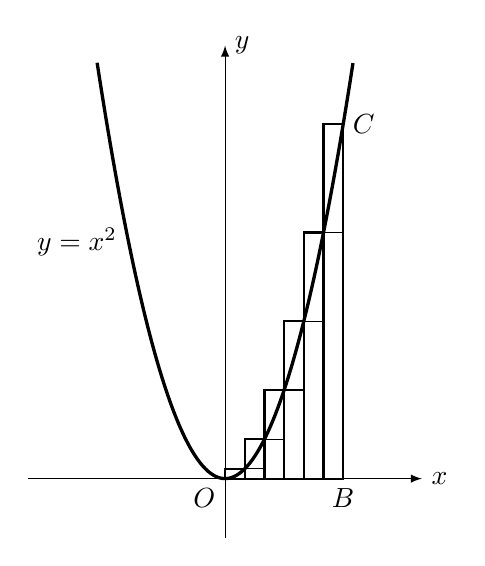
\begin{tikzpicture}[>=latex, scale=.5]
\draw[->](-5,0)--(5,0)node[right]{$x$};
\draw[->](0,-1.5)--(0,11)node[right]{$y$};
\draw[domain=-3.25:3.25, samples=100, very thick]plot(\x, {\x*\x});
\node at (0,0)[below left]{$O$};
\foreach \x in {.5,1,...,3}
{
    \draw[thick](\x-.5,0) rectangle (\x, \x*\x);
}
\foreach \x in {.5,1,...,2.5}
{
    \draw(\x,\x*\x) -- (\x+.5,\x*\x);
}
\node at (3,9)[right]{$C$};
\node at (3,0)[below]{$B$};
\node at (-2.5,6)[left]{$y=x^2$};
\end{tikzpicture}
    \caption{}
\end{figure}

\begin{solution}
\begin{enumerate}
    \item 把线段$[0,b]$ $n$等分,等分点的坐标是
   $ x_i=\frac{b}{n}i\;  (i=0, 1, 2,\ldots,n)$ 
   \item 作阶梯函数$g_n(x)$和
    $G_n (x)$.

    根据$f(x)=x^2$在$x>0$时递增,定义
\[\begin{split}
g_n(x)&=f(x_i)=x^2_i=\left(\frac{b}{n}\right)^2i^2,\quad x_i\le x<x_{i+1}\\
G_n(x)&=f(x_{i+1})=x^2_{i+1}=\left(\frac{b}{n}\right)^2(i+1)^2,\quad x_i<x\le x_{i+1}\\
\end{split}\]
其中,$i=0,1,2,\ldots,(n-1)$。于是,$g_n(x)\le f(x)\le G_n(x),\quad 0\le x\le b$

\item 求阶梯函数的和
\[\begin{split}
s_n&=g_n(x)\text{从0到$b$的和}\\
&=f\left(x_{0}\right) \cdot \frac{b}{n}+f\left(x_{1}\right) \cdot \frac{b}{n}+\cdots+f\left(x_{n-1}\right) \cdot \frac{b}{n}\\
&=\left\{f\left(x_{0}\right)+f\left(x_{1}\right)+\cdots+f\left(x_{n-1}\right)\right\} \cdot \frac{b}{n} \\
&=\left\{0^{2}+1^{2}+2^{2}+\cdots+(n-1)^{2}\right\} \cdot\left(\frac{b}{n}\right)^3\\
&=\frac{1}{6}n(n-1)(2 n-1) \cdot\left(\frac{b}{n}\right)^{3} =\frac{b^3}{6}\left(1-\frac{1}{n}\right)\left(2-\frac{1}{n}\right) 
\end{split}\]
\[\begin{split}
   S_{n}= G_{n}(x) \text { 从0到$b$的和}
   &= \left\{f\left(x_{1}\right)+f\left(x_{2}\right)+\cdots+f\left(x_{n}\right)\right\} \cdot \frac{b}{n} \\
   &=\left\{1^2+2^{2}+\cdots+n^{2}\right\} \cdot\left(\frac{b}{n}\right)^{3} \\
   &=\frac{1}{6}n(n+1)(2 n+1) \cdot\left(\frac{b}{n}\right)^{3} \\
   &=\frac{b^3}{6}\left(1+\frac{1}{n}\right)\left(2+\frac{1}{n}\right) 
\end{split}\]

综合上述计算和性质1,有:
\[\begin{split}
\frac{b^3}{6}\left(1-\frac{1}{n}\right)\left(2-\frac{1}{n}\right)&=s_n\le \begin{bmatrix}
\text{函数$f(x)=x^2$从0到$b$的和,}\\
\text{相应的曲边三角形$OBC$的面积}
\end{bmatrix}\\
&\le S_n=\frac{b^3}{6}\left(1+\frac{1}{n}\right)\left(2+\frac{1}{n}\right)
\end{split}\]

\item 令$n\to\infty$,求阶梯函数和式的极限。因为
\[\begin{split}
    \frac{b^3}{6} \left(1-\frac{1}{n}\right)\left(2-\frac{1}{n}\right)\to \frac{b^3}{3}\qquad (n\to\infty)\\
    \frac{b^3}{6} \left(1+\frac{1}{n}\right)\left(2+\frac{1}{n}\right)\to \frac{b^3}{3}\qquad (n\to\infty)\\
\end{split}\]
所以$\frac{1}{3}b^3$是能被$s_n$、$S_n$左、右夹逼的唯一实数,而所求的“$f(x)=x^2$从0到$b$的和”以及“曲边三角形$OBC$的面积,”这两个值都是夹逼在$s_n$和$S_n$中间的实数,故它们都等于$\frac{1}{3}b^3$.
\end{enumerate}
\end{solution}

\begin{blk}
    {推论} $f(x)=x^2$从$a$到$b$的和$=\frac{1}{3}b^3-\frac{1}{3}a^3\quad  (b> a> 0)$.
\end{blk}


\begin{example}
设$y=f(x)$是一个定义在$[a,b]$上的递增连续函数,试说明它从$a$到$b$的和是可以确定的。
\end{example}

\begin{figure}[htp]
    \centering
\begin{tikzpicture}[>=latex]
\draw[->](-.5,0)--(5,0)node[right]{$x$};
\draw[->](0,-.5)--(0,4)node[right]{$y$};
\draw[domain=.5:4, samples=50, very thick]plot(\x, {.2*\x*\x+.5});
\draw[dashed](1,.7)--(1,0)node[below]{$a$};
\draw[dashed](4,3.7)--(4,0)node[below]{$b$};
\draw[dashed](2,1.3)--(2,0);
\draw[dashed](3,2.3)node[left]{$y=f(x)$}--(3,0);
\node at (0,0)[below left]{$O$};
\end{tikzpicture}
    \caption{}
\end{figure}

\begin{solution}
\begin{enumerate}
    \item     取$[a,b]$之间的$n$等分点,将它分成$n$段,即有
\[x_0=a<x_1<x_2<\cdots<x_n=b\]
它的第$i$段是$[x_{i-1},x_i]$,且$x_i-x_{i-1}=\frac{b-a}{n}$,$x_i=a+\frac{i}{n}(b-a)$

\item 定义$f(x)$的上、下夹逼阶梯函数如下:
\[\begin{split}
    g_n(x)&=f(x_{i-1}),\qquad x_{i-1}\le x\le x_i \\
    G_n(x)&=f(x_i),\qquad x_{i-1}\le x\le x_i 
\end{split}(i=1,2,3,\ldots,n)\]
由$f(x)$的递增性,对于任何一个$x\in[a,b]$,有
\[g_1(x)\le g_2(x)\le\cdots \le g_n(x)\le\cdots \le f(x)\le \cdots\le G_n(x)\le\cdots\le G_2(x)\le G_1(x)\]
简写成
\[g_n(x)\le f(x)\le G_n(x),\qquad a\le x\le b\]
\item 求相应的阶梯函数从$a$到$b$的和
\begin{equation}
\begin{split}
    s_n=g_n(x)\text{从$a$到$b$的和}
    &=\frac{b-a}{n}\left[f(x_0)+f(x_1)+\cdots+f(x_{n-1})\right]\\
    &=\frac{b-a}{n}\sum^n_{i=1}f(x_{i-1})
\end{split}
\end{equation}
\begin{equation}
    \begin{split}
    S_n=G_n(x)\text{从$a$到$b$的和}
    &=\frac{b-a}{n}\left[f(x_1)+f(x_2)+\cdots+f(x_{n})\right]\\
    &=\frac{b-a}{n}\sum^n_{i=1}f(x_{i})   
    \end{split}
    \end{equation}
\end{enumerate}
由性质1, 有:
\[s_1<s_2<\cdots<s_n<\cdots<f(x)\text{从$a$到$b$的和}<\cdots<S_n<\cdots<S_2<S_1\]
简写成
\begin{equation}
    s_n<f(x)\text{从$a$到$b$的和}<S_n
\end{equation}
在例3.3, 例3.4中,$f(x)$有明确的解析式,我们可以用求和公式直接求出$s_n$和$S_n$的表达式,从而可以得出它们的共同极限值,在这里,我们只知道$f(x)$的递增性,当然无法将和式$s_n$和$S_n$进一步化简,但是我们可以说明,当$n\to\infty$时,$S_n-s_n\to 0$.

事实上,
\[\begin{split}
    S_n-s_n&=\frac{b-a}{n}\sum^n_{i=1}f(x_{i})   -\frac{b-a}{n}\sum^n_{i=1}f(x_{i-1}) \\
    &=\frac{b-a}{n}\sum^n_{i=1}\left[f(x_{i})-f(x_{i-1})\right]   \\
    &=\frac{b-a}{n}\left[f(x_{n})-f(x_{0})\right]  =\frac{b-a}{n}\left[f(b)-f(a)\right]   
\end{split}\]
因此,当$n\to\infty$时,$S_n-s_n\to 0$.

又$f(x)$从$a$到$b$的和是介于$s_n$和$S_n$中间的唯一实数,
此
\[\lim_{n\to\infty} s_n=\lim_{n\to\infty} S_n=f(x)\text{ 从$a$到$b$的和}\]

以上简单明了的分析,说明了下面两点互相关联的事实:
\begin{enumerate}
    \item 当函数$f(x)$在$a\le x\le b$上递增时,则它从$a$到$b$的和可以用上述两个夹逼阶梯函数从$a$到$b$的和去无限逼近.
    \item 由于$\Lim_{n\to\infty}s_n$与$\Lim_{n\to\infty}S_n$存在,且$\Lim_{n\to\infty}s_n=\Lim_{n\to\infty}S_n$, 我们可以用$f(x)$的上、下夹逼阶梯函数序列,即:$g_1 (x)\le g_2(x)\le \cdots\le g_n(x)\le \cdots\le f(x)\le \cdots\le G_1(x)\le \cdots\le G_2(x)\le G_1(x),\; (a\le x\le b)$的从$a$到$b$的和的极限$\Lim_{n\to\infty}s_n=\Lim_{n\to\infty}S_n$作为上述$f(x)$从$a$到$b$的和的数量化定义。
\end{enumerate}
\end{solution}

\begin{blk}
    {定义1}若$f(x)$是$[a,b]$上的递增连续函数,将$[a,b]$等分成$n$段,分点坐标$x_i=a+\frac{i}{n}(b-a),\; i=0,1, 2,\ldots,n$,则存在两个阶梯函数:
\[    g_n (x) =f (x_{i-1}) ,\quad x_{i-1}\le  x< x_i\]
    和
\[    G_n (x)=f(x_i),\quad x_{i-1}<x\le x_i,\quad (i=1,2,\ldots,n)\]
满足下面的性质:
\begin{enumerate}
    \item 对于任何$x\in[a,b]$,$g_n(x)\le f(x)\le G_n(x)$
    \item 相应的阶梯函数从$a$到$b$的和
\[s_n=\frac{b-a}{n}\sum^n_{i=1}f(x_{i-1}),\qquad S_n=\frac{b-a}{n}\sum^n_{i=1}f(x_{i})  \]
\end{enumerate}
当$n\to\infty$时,$S_n-s_n\to 0$,那么$f(x)$从$a$到$b$的和是$s_n$与$S_n$的共同极限,即:
\[\begin{split}
f(x)\text{从$a$到$b$的和}&=\frac{b-a}{n}\lim_{n\to\infty}\sum^n_{i=1}f(x_{i-1})\\
&=\frac{b-a}{n}\lim_{n\to\infty}\sum^n_{i=1}f(x_{i})
\end{split}\]

同样地,如果$f(x)$是$[a,b]$上的递减连续函数。那么将$[a,b]$ $n$等分,分点坐标$x_i=a+\frac{i}{n}(b-a)$, 这时有两个阶梯函数
\[    g_n (x) =f (x_{i}) ,\quad x_{i-1}<  x\le x_i\]
    和
\[    G_n (x)=f(x_{i-1}),\quad x_{i-1}\le x< x_i,\quad (i=1,2,\ldots,n)\]
满足下面的性质:
\begin{enumerate}
    \item 对于任何$x\in[a,b]$,$g_n(x)\le f(x)\le G_n(x)$
    \item 相应的阶梯函数$g_n(x)$与$G_n(x)$相应的和
\[\begin{split}
    s_n&=g_n\text{从$a$到$b$的和}=\frac{b-a}{n}\sum^n_{i=1}f(x_{i})\\
    S_n&=G_n\text{从$a$到$b$的和}=\frac{b-a}{n}\sum^n_{i=1}f(x_{i-1})  
\end{split}\]
\end{enumerate}
当$n\to\infty$时,$S_n-s_n=\frac{b-a}{n}\left[f(b)-f(a)\right]\to 0$,即:
\[\Lim_{n\to\infty}s_n=\Lim_{n\to\infty}S_n\]
\end{blk}

\begin{blk}
    {定义2} 递减连续函数从$a$到$b$的和为上述夹逼阶梯函数$g_n(x)$和$G_n(x)$从$a$到$b$的和的共同极限,即  
\[\begin{split}
    f(x)\text{从$a$到$b$的和}&=\lim_{n\to\infty} \frac{b-a}{n}\sum^n_{i=1}f(x_i)\\
    &=\lim_{n\to\infty} \frac{b-a}{n}\sum^n_{i=1}f(x_{i-1})\\
\end{split}\]
\end{blk}

通常我们把递增或递减的函数合称为单调函数,常见的
函数$f(x)$都是分段单调连续的,例如,$y=\sin x$本身虽然不是单调的,但是它在$\left[-\frac{\pi}{2}+2k\pi,\frac{\pi}{2}+2k\pi\right]\; (k\in\mathbb{Z})$这些区间的每一段是递增的;而在$\left[\frac{\pi}{2}+2k\pi,\frac{3\pi}{2}+2k\pi\right]\; (k\in\mathbb{Z})$这些区间的每一段是递减的。因此,对于一般在$[a,b]$上连续的函数,如果存在有限个分点使得$f(x)$在每个分段上都是单调的,我们可以逐段取上、下夹逼阶梯函数,合起来作为定义在$[a,b]$上的函数$f(x)$的阶梯函数,于是得出
\[g_n (x)\le f(x)\le G_n(x),\qquad x\in [a,b]\]
又因为有限个在分段上趋于0的量的和仍趋于0, 所以
\[\text{“$G_n(x)$从$a$到$b$的和”}-\text{“$g_n(x)$从$a$到$b$的和”}\to 0\]

总结以上讨论,我们叙述为存在定理和定义如下:

\begin{blk}
    {定理} 设$y=f(x)$是一个定义在$[a,b]$上分段单调函数,则存在满足下列性质的两系列阶梯函数:
    \[g_n(x)\le f(x)\le G_n(x),\qquad x\in[a,b]\]
而且当$n\to 0$时,“$G_n(x)$从$a$到$b$的和,”与“$g_n(x)$从$a$到$b$的和”趋于共同极限。
\end{blk}


\begin{blk}
    {定义3} 设$f(x)$是$[a,b]$上的连续函数,如果 存在有限个分点:
\[a=a_0<a_1<\cdots<a_k<\cdots<a_1=b\]
使得$f(x)$在每个分段$[a_{k-1},a_k]$都是单调的,再将每个分段
    $[a_{k-1},a_k]$都$n$等分,则当$n\to\infty$时,有
\[\begin{split}
f(x)\text{从$a$到$b$的和}&=\lim_{n\to\infty}\frac{a_1-a_0}{n}\sum^n_{i=1}f(x_i)+\lim_{n\to\infty}\frac{a_2-a_1}{n}\sum^{2n}_{i=n+1}f(x_i)+\\
&\cdots +\lim_{n\to\infty}\frac{a_\ell-a_{\ell-1}}{n}\sum^{\ell n}_{i=\ell(n-1)+1}f(x_i)
\end{split}\]
\end{blk}

为了说明上述定义是合理的,我们就得证明上述$f(x)$从$a$到$b$的和与夹逼的阶梯函数列$\{G_n(x)\}$和$\{g_n(x)\}$的选取无关,其证明如下:

\begin{proof}
    设$\{\bar G_m(x)\}$和$\{\bar g_m(x)\}$是另外一组满足存在定理的上、下夹逼函数列,则由下述不等式
\[g_n(x)\le f(x)\le G_n(x),\quad \bar g_m(x)\le f(x)\le \bar G_m(x),\qquad a\le x\le b\]
即有
\[g_n(x)\le \bar G_m(x),\qquad \bar g_m(x)\le G_n(x)\]
所以由基本性质1,有
\[\begin{split}
    s_n&=g_n(x)\text{从$a$到$b$的和}\le \bar G_m(x)\text{从$a$到$b$的和}=\bar S_m\\
    \bar s_m&=\bar g_m(x)\text{从$a$到$b$的和}\le G_n(x)\text{从$a$到$b$的和}=S_n\\
\end{split}\]
所以
\[\lim_{n\to\infty}s_n=\lim_{m\to\infty}\bar S_m,\qquad \lim_{m\to\infty}\bar s_m\le \lim_{n\to\infty}S_n\]
但是
\[\lim_{n\to\infty}s_n\le \lim_{m\to\infty}\bar S_m=\lim_{m\to\infty}\bar s_m\le \lim_{n\to\infty} S_n=\lim_{n\to\infty}s_n\]
所以上述极限必须相等,即:
\[\lim_{n\to\infty}s_n= \lim_{m\to\infty}\bar S_m=\lim_{m\to\infty}\bar s_m=\lim_{n\to\infty} S_n\]
\end{proof}

\begin{example}
求$f(x)=2x-x^2$从0到2的和.
\end{example}

\begin{solution}
    由$f'(x)=2-2x$, $f''(x)=2$知$f(1)=2-1=1$是
$f(x)$的极大值,并且$y=2x-x^2$在$[0, 1]$上递增,在$[1,2]$上递减,于是,我们把区间$[0, 1]$和$[1, 2]$都$n$等分,设分点坐标$x_i=\frac{i}{n},\; i=0, 1, 2,\ldots,2n$, 即有
\[0=x_0<x_1<x_2<\cdots <x_n=1<x_{n+1}<x_{n+2}<\cdots <x_{2n}=2\]
且$\Delta x_i=x_i-x_{i-1}=\frac{1}{n}$,由定义3得到:
\[\begin{split}
    f(x)&=2x-x^2\text{从0到2的和}\\
    &=\lim_{n\to\infty}\frac{1}{n}\sum^n_{i=1}\left[2\left(\frac{i}{n}\right)-\left(\frac{i}{n}\right)^2\right]+\lim_{n\to\infty}\frac{1}{n}\sum^{2n}_{i=n+1}\left[2\left(\frac{i}{n}\right)-\left(\frac{i}{n}\right)^2\right] \\
&=\lim_{n\to\infty}\frac{1}{n}\sum^{2n}_{i=1}2\left(\frac{i}{n}\right)-\lim_{n\to\infty}\sum^{2n}_{i=1}\left(\frac{i}{n}\right)^2\\
&=2\lim_{n\to\infty}\frac{1}{n^2}\sum^{2n}_{i=1}i-\lim_{n\to\infty}\frac{1}{n^3}\sum^{2n}_{i=1}i^2\\
&=2\lim_{n\to\infty}\frac{1}{n^2}\cdot \frac{(2n+1)2n}{2}-\lim_{n\to\infty}\frac{1}{n^3}\cdot \frac{2n(2n+1)(4n+1)}{6}\\
&=2\lim_{n\to\infty}\left(2+\frac{1}{n}\right)-\lim_{n\to\infty}\frac{1}{3}\left(2+\frac{1}{n}\right)\left(4+\frac{1}{n}\right)\\
&=4-\frac{8}{3}=\frac{4}{3}
\end{split}\]
\end{solution}

\begin{ex}
\begin{enumerate}
    \item 已知质点的运动速度$v=t+4$, 试求质点在前10秒内所走的路程。
    \item 求$f(x)=x^3$在$1\le x\le 2$上的和。
\end{enumerate}
\end{ex}


\section{定积分的定义和基本性质}
\subsection{定积分定义}

设函数$f(x)$在$[a,b]$上连续,如果存在有限个分点
\[a=a_0<a_1<a_2<\cdots<a_{\ell-1}<a_{\ell}=b\]
使得$f(x)$在每个分段$[a_{k-1},a_k]\; (k=1, 2,\ldots,\ell)$上都是单调的,我们把$f(x)$从$a$到$b$的和叫做$f(x)$从$a$到$b$的\textbf{定积分},并记作
\[\int^b_a f(x) \dd x\]

这里,积分符号所使用的是长$S$形的求和号的变形,而从部分区间长$\Delta x_i=\frac{a_k-a_{k-1}}{n}$过渡到极限,则通过字母$\dd$来表示。

我们把数$a$与$b$称为\textbf{积分限}($a$称为\textbf{下限},$b$称为\textbf{上限})。区间$[a,b]$称为\textbf{积分区间},函数$f(x)$称为\textbf{被积函数},乘积$f(x)\dd x$称为\textbf{被积表达式},定积分符号下出现的字母$x$叫做\textbf{积分变量}。

上述定积分定义用定积分符号表示就是:
\[\int^b_a f(x) \dd x=\sum^t_{k=1}\int^{a_k}_{a_{k-1}}f(x)\dd x\]
其中$\Int^{a_k}_{a_{k-1}}f(x)\dd x$是$f(x)$为单调的第$k$个分段$[a_{k-1},a_k]$上的夹逼阶梯函数$g_n(x)$和$G_n(x)$从$a_{k-1}$到$a_k$的和的共同极限,即:
\[\begin{split}
    \int^{a_k}_{a_{k-1}}f(x)\dd x&=\lim_{n\to \infty}\frac{a_k-a_{k-1}}{n}\sum^n_{i=1}f(x_{i-1})\\
    &=\lim_{n\to \infty}\frac{a_k-a_{k-1}}{n}\sum^n_{i=1}f(x_{i})
\end{split}\]

定积分定义的另一种表述形式是:设函数$f(x)$在$a\le x\le b$上分段单调连续,如果存在两系列上、下夹逼阶梯函数$\{g_n(x)\}$, $\{G_n(x)\}$, 使得
\[g_n (x)\le f(x)\le G_n(x),\qquad a\le x\le b\]
并且$g_n(x)$从$a$到$b$的和$s_n$与$G_n(x)$从$a$到$b$的和$S_n$具有相同的
极限,这个极限叫做$f(x)$从$a$到$b$的定积分$\Int^b_a f(x) \dd x$.

综上所述,在积分符号中,我们只对$a<b$, 即积分下限小于积分
上限的情形给出了定义,若$a>b$,我们定义
\[\int^a_b f(x) \dd x=-\int^b_a f(x) \dd x\]
此外,由于定积分可以解释为曲边梯形的面积,自然可以定
\[\int^a_a f(x) \dd x=0\]
作了这样的规定之后,不论$a<b$, $a>b$或$a=b$, 定积分都有意义了。


\begin{ex}
\begin{enumerate}
    \item 求证 $\Int_{a}^{b} k x\dd x=\frac{k b^{2}}{2}-\frac{k a^{2}}{2} \quad(a<b)$
    \item  求 $\Int_{8}^{0}\left(x^{2}-4 x\right) \dd x$
    \item  求 $\Int_{-1}^{2}\left(x^{3}-3 x\right) \dd x$
\end{enumerate}
\end{ex}

\subsection{逼近法求曲线形的面积}

任意一条曲线围成的图形(图3.11)常常可以用两组互相垂直的直线把它分成若干部分,每一部分都是一个曲边梯形(图3.12), 在这里并不排除下述情形(图3.13):两条平行的边中有一条缩成了一点,因而曲边梯形变成了曲边三角形,这样一来,我们的问题就化成了求曲边梯形面积的问题。

\begin{figure}[htp]
    \centering
    \begin{minipage}[t]{0.45\textwidth}
        \centering
        \begin{tikzpicture}[>=latex, scale=1]
    \draw(-2,3)--(2,3);
    \draw(-2,2)--(2,2); 
    \draw(-.5,0)--(-.5,4);
    \draw(.5,0)--(.5,4); 
    \node at (0,0){
\pscurve(-0.32,3.56)(-0.82,3.36)(-1.12,2.9)(-1.42,1.72)(-1.26,0.9)(-1.08,0.78)(-0.64,0.64)(-0.56,0.64)(-0.5,0.62)(-0.42,0.62)(-0.36,0.6)(-0.3,0.58)(0.1,0.5)(0.18,0.5)(0.24,0.52)(0.48,0.7)(0.64,0.86)(0.7,0.9)(1.36,1.62)(1.42,1.7)(1.36,3.16)(0.96,3.56)(0.84,3.66)(0.78,3.7)(0.6,3.8)(0.54,3.82)(0.34,3.82)(-0.32,3.56)
};

        \end{tikzpicture}
        \caption{}
        \end{minipage}
    \begin{minipage}[t]{0.25\textwidth}
    \centering
    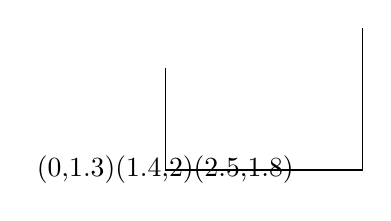
\begin{tikzpicture}[>=latex, scale=1]
    \draw(0,1.3)--(0,0)--(2.5,0)--(2.5,1.8);
    \node at (0,0){
\pscurve(0,1.3)(1.4,2)(2.5,1.8)
};
    \end{tikzpicture}
    \caption{}
    \end{minipage}
    \begin{minipage}[t]{0.25\textwidth}
    \centering
    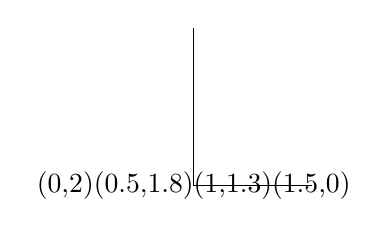
\begin{tikzpicture}[>=latex, scale=1]
    \draw(0,2)--(0,0)--(1.5,0);
    \node at (0,0){
\pscurve(0,2)(0.5,1.8)(1,1.3)(1.5,0)
};
    \end{tikzpicture}
    \caption{}
    \end{minipage}
  \end{figure}

\begin{blk}
  {命题} 设$y=f(x)$是定义在$a\le x\le b$的分段单调连续函数,而且$f(x)\ge 0$, 则区域$R=\{a\le x\le b,\; 0\le y\le f(x)\}$的
面积等于
\[\int^b_a f (x) \dd x \]  
\end{blk}

\begin{figure}[htp]
    \centering
\begin{tikzpicture}[>=latex]
    \draw[->, thick](-.5,0)--(7,0)node[right]{$x$};
    \draw[->, thick](0,-.5)--(0,5)node[right]{$y$};
\draw[domain=.5:6, samples=100, very thick]plot(\x, {1.5*sin(1.2*(\x-1) r)+3});
\draw(.5,0)node[below]{$a$} rectangle  (1.1, .18+3);
\draw(1.1,0) rectangle  (1.8, 1.23+3);
\draw(1.8,0) rectangle  (2.5, 1.46+3);
\draw[pattern=north east lines](2.5,0) rectangle  (3.5, .212+3);
\draw[pattern=north east lines](3.5,0) rectangle  (4.2, -.965+3);
\draw[pattern=north east lines](4.2,0) rectangle  (5, -1.49+3);
\draw(5,0) rectangle  (5.5, -1.16+3);
\draw(5.5,0) rectangle (6, -.419+3);

\draw[pattern=north east lines](.5,0) rectangle  (1.1, -.847+3);
\draw[pattern=north east lines](1.1,0) rectangle  (1.8, .18+3);
\draw[pattern=north east lines](1.8,0) rectangle  (2.5, 1.23+3);
\draw(2.5,0) rectangle  (3.5, 1.46+3);
\draw(3.5,0) rectangle  (4.2, .212+3);
\draw(4.2,0) rectangle  (5, -.965+3);
\draw[pattern=north east lines](5,0) rectangle  (5.5,-1.49+3);
\draw[pattern=north east lines](5.5,0) rectangle (6, -1.16+3);

\node at (6,0)[below]{$b$};
\node at (0,0)[below left]{$O$};
\node at (4.5,3.2)[above]{$y=f(x)$};

\end{tikzpicture}
    \caption{}
\end{figure}


\begin{proof}
    由$\Int^b_a f (x) \dd x$的定义得知,存在两系列阶梯函数
$\{g_n(x)\}$和$\{G_n(x)\}$, 满足下面的性质:
\[g_n(x)\le f (x) \le G_n(x)\]
而且$G_n(x)$从$a$到$b$的和与$g_n(x)$从$a$到$b$的和趋于共同的极限$\Int^b_a f (x) \dd x$. 令
\[\begin{split}
    R_n&=\{a\le x\le b,\; 0\le y\le g_n(x)\}\\
    R'_n&=\{a\le x\le b,\; 0\le y\le G_n(x)\}\\
\end{split}\]
它们都是由高高低低的狭长方形所组成的区域(图3.14),则:
\[R_n\subset \text{曲边梯形区域 }R \subset R'_n\]
而且
\[R_n\text{的面积}=g_n(x)\text{从$a$到$b$的和}s_n,\qquad R'_n\text{的面积}=G_n(x)\text{从$a$到$b$的和}S_n\]
即有
\[s_n<\text{曲边梯形区域$R$的面积}A<S_n\]
由定积分定义有:
\[\lim_{n\to\infty}s_n=\lim_{n\to\infty}S_n=\Int^b_a f (x) \dd x\]
又曲边梯形面积$A=(f,\; [a,b])$也是夹逼在$s_n$和$S_n$中间的实数,所以
\[A=(f,\; [a,b])=\Int^b_a f (x) \dd x\]
\end{proof}

\begin{ex}
\begin{enumerate}
    \item 求$\Int^1_{-2}e^x\dd x$. 

提示:$\frac{e^{\Delta x}-1}{\Delta x}=1$.    

\item 求在$x=0$与$x=\pi$间正弦曲线$y=\sin x$与$Ox$轴所包的面积。
\end{enumerate}
\end{ex}    

\subsection{定积分的基本性质}

为简单起见,我们约定以下被积函数在积分区间上连续并且可以分段单调,即$f(x)$是在$[a,b]$上连续并且只有有限个极大值和极小值的函数。

\begin{blk}{性质1}
若$a<b<c$,那么,
\[\int^b_a f(x)\dd x+\int^c_b f(x)\dd x=\int^c_a f(x)\dd x\]
\end{blk}

\begin{proof}
因为$\Int^b_a f(x)\dd x$存在,故对于在$[a,b]$上的
$f(x)$, 存在一组上、下夹逼函数列$\{g_n(x)\}$和$\{G_n(x)\}$, 使得
\[g_n (x) \le f (x) \le G_n (x),\qquad x\in [a,b]\]
且相应的阶梯函数在$[a,b]$上的和$s_n$与$S_n$适合
\begin{equation}
    s_n<\int^b_a f(x)\dd x<S_n,\qquad S_n-s_n\to 0
\end{equation}
对于在$[b,c]$上的$f(x)$, 同样得到
\[\bar g_n (x) \le f (x) \le \bar G_n (x),\qquad x\in [b,c]\]
且
\begin{equation}
    \bar  s_n<\int^c_b f(x)\dd x<\bar S_n,\qquad \bar S_n-\bar s_n\to 0
\end{equation}
$(3.4)+(3.5)$得到
\begin{equation}
    s_n+ \bar  s_n<\int^b_a f(x)\dd x+\int^c_b f(x)\dd x<S_n+\bar S_n
\end{equation}

另一方面,对于函数$f(x)\; (a\le x\le c)$存在下面一组阶梯函数列:
\[\tilde g_n(x)=\begin{cases}
    g_n(x),  &  a\le x\le b\\
    \max\left(g_n(b), \bar g_n(b)\right),  &  x=b\\
    \bar g_n(x), & b<x\le c
\end{cases}\]
\[\tilde G_n(x)=\begin{cases}
    G_n(x),  &  a\le x\le b\\
    \max\left(G_n(b), \bar G_n(b)\right),  &  x=b\\
    \bar G_n(x), & b<x\le c
\end{cases}\]

由性质2,阶梯函数列$\tilde g_n(x)$与$\tilde G_n(x)$的从$a$到$c$的和分别是$s_n+\bar s_n$和$S_n+\bar S_n$。因为$\tilde g_n(x)$与$\tilde G(x)$满足条件:
\begin{enumerate}
    \item $\tilde g_n(x)\le f(x)\le \tilde G(x),\quad a\le x\le c$
    \item \[\begin{split}
    \lim_{n\to\infty}\left[(S_n+\bar S_n)-(s_n+\bar s_n)\right]&=\lim_{n\to\infty}\left[(S_n-s_n)+(\bar S_n-\bar s_n)\right]\\
    &=\lim_{n\to\infty}(S_n-s_n)+\lim_{n\to\infty}(\bar S_n-\bar s_n)=0
    \end{split}\]
\end{enumerate}
所以根据定积分定义得到
\[\lim_{n\to\infty}(S_n+\bar S_n)=\lim_{n\to\infty}(s_n+\bar s_n)=\int^c_a f(x)\dd x \]

因为$\Int^c_a f(x)\dd x $与$\Int^b_a f(x)\dd x +\Int^c_b f(x)\dd x $都是被$s_n+\bar s_n$与$S_n+\bar S_n$所夹逼的唯一实数,所以
\[\Int^c_a f(x)\dd x=\Int^b_a f(x)\dd x +\Int^c_b f(x)\dd x\]
\end{proof}

\begin{blk}{性质2}
若$f(x)=f_1(x)+f_2(x)$,则:
\[\Int^b_a f(x)\dd x=\Int^b_a f_1(x)\dd x +\Int^b_a f_2(x)\dd x\]
\end{blk}

\begin{proof}
设$\{g_n(x)\}$与$\{G_n(x)\}$是$f_1(x)$在$[a,b]$上的上、下夹逼阶梯函数列,又$\{\bar g_n(x)\}$与$\{\bar G_n(x)\}$是$f_2(x)$在$[a,b]$上的上、下夹逼阶梯函数列。$s_n, S_n, \bar s_n, \bar S_n$是相应的阶梯函数从$a$到$b$的和。于是由
$\Int^b_a f_1(x)\dd x$和$\Int^b_a f_2(x)\dd x$的存在,得:
\begin{align}
g_n(x)\le f_1(x)\le G_n(x),\qquad a\le x\le b\\
\bar g_n(x)\le f_2(x)\le \bar G_n(x),\qquad a\le x\le b
\end{align}
并且
\begin{align}
s_n<\Int^b_a f_1(x)\dd x<S_n,\quad \text{且 } S_n-s_n\to 0\\
\bar s_n<\Int^b_a f_2(x)\dd x<\bar S_n,\quad \text{且 } \bar S_n-\bar s_n\to 0
\end{align}
由$(3.9)+(3.10)$,得到
\begin{equation}
   s_n+ \bar s_n <\Int^b_a f_1(x)\dd x+\Int^b_a f_2(x)\dd x<S_n+\bar S_n
\end{equation}
另一方面,由$(3.7)+(3.8)$,得到
\[g_n(x)+\bar g_n(x)\le f_1(x)+ f_2(x)\le G_n(x)+\bar G_n(x),\qquad a\le x\le b\]
而且,$g_n(x)+\bar g_n(x)$与$G_n(x)+\bar G_n(x)$也是在$[a,b]$上的阶梯函数,我们要说明它们是$f_1(x)+ f_2(x)$在$[a,b]$上的一组夹逼阶梯函数列。

因为:
\[\begin{split}
    g_n(x)+\bar g_n(x)\text{从$a$到$b$的和}&=\left[ g_n(x)\text{从$a$到$b$的和}\right]+\left[\bar g_n(x)\text{从$a$到$b$的和}\right]\\
    &=s_n+\bar s_n\\
    G_n(x)+\bar G_n(x)\text{从$a$到$b$的和}&=\left[ G_n(x)\text{从$a$到$b$的和}\right]+\left[\bar G_n(x)\text{从$a$到$b$的和}\right]\\
    &=S_n+\bar S_n
\end{split}\]
而且
\begin{equation}
    \left(S_n+\bar S_n\right)-\left(s_n+\bar s_n\right)=\left(S_n-s_n\right)+\left(\bar S_n-\bar s_n\right)\to 0
\end{equation}
所以,由$\Int^b_a \bigl(f_1(x)+ f_2(x)\bigr)\dd x$的定义,得到
\begin{equation}
    \lim_{n\to\infty}\left(S_n+\bar S_n\right)=\lim_{n\to\infty}\left(s_n+\bar s_n\right)=\Int^b_a \bigl(f_1(x)+ f_2(x)\bigr)\dd x
\end{equation}
由(3.10)和(3.13),$\Int^b_a \bigl(f_1(x)+ f_2(x)\bigr)\dd x$与$\Int^b_a f_1(x)\dd x + \Int^b_a  f_2(x)\dd x$
是被$s_n+\bar s_n$与$S_n+\bar S_n$所夹逼的唯一实数,所以
\[\Int^b_a \bigl(f_1(x)+ f_2(x)\bigr)\dd x=\Int^b_a f_1(x)\dd x + \Int^b_a  f_2(x)\dd x\]
\end{proof}

\begin{blk}{性质3}
\[\Int^b_a kf(x)\dd x =k\Int^b_a f(x)\dd x \]
\end{blk}

此法则的证明大致和性质2的证明相同,即当$\{g_n(x)\}$和$\{G_n(x)\}$上、下夹逼$f(x)$时,那么在$k>0$的情形,$\{kg_n(x)\}$和$\{kG_n(x)\}$上、下夹逼$kf(x)$; 在$k<0$的情形,$\{kg_n(x)\}$和$\{kG_n(x)\}$上、下夹逼$kf(x)$. 我们把证明的过程留给读者去写。

\begin{blk}{性质4}
    若$m\le f(x)\le M$, $a\le x\le b$,那么
    \[m(b-a)\le \Int^b_a f(x)\dd x \le M(b-a) \]
    \end{blk}

\begin{proof}
    设$\{g_n(x)\}$与$\{G_n(x)\}$是$f(x)$在$[a,b]$上的夹逼阶梯函数列,$s_n$与$S_n$是相应的阶梯函数在$[a,b]$上的和,根据积分的定义,有
\[\lim_{n\to\infty}s_n=\lim_{n\to\infty}S_n=\int^b_a f(x)\dd x\]
换言之,任给一个正数$\varepsilon$,存在自然数$N$,使得当$n<N$时,有
\begin{equation}
    S_n<\int^b_a f(x)\dd x+\varepsilon
\end{equation}
成立。

又由于$G_n(x)\ge f(x)\ge m,\quad x\in[a,b]$,根据性质1,得到:
\begin{equation}
    S_n\ge m(b-a)
\end{equation}
所以,当$n>N$时,由(3.14)和(3.15),有
\[m(b-a)\le S_n<\int^b_a f(x)\dd x+\varepsilon\]
即
\begin{equation}
    m(b-a)<\int^b_a f(x)\dd x+\varepsilon
\end{equation}
成立。

因为这个不等式(3.16)对于每个正数$\varepsilon$都成立,所以
\[m(b-a)\le \int^b_a f(x)\dd x\]
同样证明,得到
\[M(b-a)\ge \int^b_a f(x)\dd x\]
因此
\[m(b-a)\le \int^b_a f(x)\dd x\le M(b-a)\]
\end{proof}

\begin{figure}[htp]
    \centering
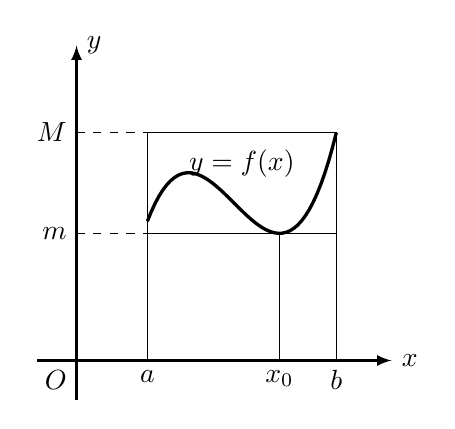
\begin{tikzpicture}[>=latex]
\draw[->, thick](-1.5,0)--(3,0)node[right]{$x$};
\draw[->, thick](-1,-.5)--(-1,4)node[right]{$y$};
\node at (-1,0)[below left]{$O$};
\draw[domain=-.1:2.3, samples=50, very thick]plot(\x, {\x*(\x-1)*(\x-2)+2});
\draw(-.1,0)node[below]{$a$} rectangle (2.3,2.9);
\node at (2.3,0)[below]{$b$};
\draw(1.577,0)node[below]{$x_0$}--(1.577,1.615);
\draw(-.1,1.615)--(2.3,1.615);
\draw[dashed](-1,1.615)node[left]{$m$}--(-.1,1.615);
\draw[dashed](-1,2.9)node[left]{$M$}--(-.1,2.9);

\node at (1.1,2.5){$y=f(x)$};
\end{tikzpicture}
    \caption{}
\end{figure}

从几何图形来看,以曲线$y=f(x)$为一边而以线段$[a,b]$为底边的曲边梯形界于以$[a,b]$为底边,高分别等于$m$和$M$的两个矩形之内,
故曲边梯形的面积$\Int^b_a f(x)\dd x$
在两个矩形面积$m(b-a)$和$M(b-a)$之间(图3.14)。

这个性质是说分段单调的连续函数$f(x)$在区间$[a,b]$上的定积分是有界的。

\begin{blk}{性质5}
如果$f(x)\le \varphi(x),\; a\le x\le b$,那么:
\[\int^b_a f(x)\dd x\le \int^b_a \varphi(x)\dd x\]
\end{blk}

\begin{proof}
    设$\{g_n(x)\}$与$\{G_n(x)\}$是$f(x)$在$[a,b]$上的夹逼阶梯函数列,又$\{\bar g_n(x)\}$与$\{\bar G_n(x)\}$是$\varphi(x)$在$[a,b]$上的夹逼阶梯函数列,
又$s_n, S_n, \bar s_n, \bar S_n$是相应的阶梯函数从$a$到$b$的和。于是根据定积分的定义,有:
\[s_n<\int^b_a f(x)\dd x<S_n,\qquad \bar s_n<\int^b_a \varphi(x)\dd x<\bar S_n\]
当$n\to\infty$时,得到:
\[\begin{split}
\lim_{n\to\infty}S_n =\lim_{n\to\infty}s_n =\int^b_a f(x)\dd x\\
\lim_{n\to\infty}\bar S_n =\lim_{n\to\infty}\bar s_n =\int^b_a \varphi(x)\dd x\\
\end{split}\]
换言之,任给正数$\varepsilon$,存在$N_1$,使得当$n>N_1$时,有
\[s_n>\int^b_a f(x)\dd x-\frac{\varepsilon}{2}\]

当$n>N_2$时,有
\[\bar s_n<\int^b_a \varphi(x)\dd x+\frac{\varepsilon}{2}\]

因为$\bar G_n(x)>\varphi(x)>f(x)>g_n(x),\quad x\in[a,b]$,根据性质1,得到:$\bar S_n=s_n$.

所以,当$n>\max(N_1,N_2)$时,有
\[\int^b_a f(x)\dd x<s_n+\frac{\varepsilon}{2}<\bar S_n+\frac{\varepsilon}{2}<\int^b_a \varphi(x)\dd x+\varepsilon\]
因为这个不等式对于每个正数$\varepsilon$都成立,所以必然有
\[\int^b_a f(x)\dd x\le \int^b_a \varphi(x)\dd x\]
\end{proof}

\begin{blk}{性质6:定积分中值定理}
   设函数$f(x)$在闭区间$[a,b]$上分段单调连续,又
$m=f(c)$, $M=f(d)$分别是$f(x)$在$[a,b]$上的最小值和最大值,则在$[a,b]$上至少存在一点$\xi$, 使得下面的等式成立:
\[\int^b_a f (x) \dd x=f(\xi) (b-a)\] 
\end{blk}

\begin{proof}
    因为$m\le f (x) \le M,\quad x\in [a,b]$, 
由性质4, 即得
\[m (b-a)\le \int^b_a f (x) \dd x\le M(b-a)\]
上面不等式的两端各除以$(b-a)$, 得
\[f(c)=m\le \frac{\int^b_a f (x) \dd x}{b-a}\le M=f(d)\]
因为$f(x)$在$[a,b]$上连续,再由连续函数的中间值定理,必存在一个$\xi\in(c,d)$, 使得
\[f(\xi)=\frac{1}{b-a}\int^b_a f (x) \dd x\]
两边再乘以$(b-a)$,得
\[\int^b_a f (x) \dd x=f(\xi)(b-a)\]
这就是我们所要证明的。
\end{proof}

这个公式的几何意义是:以线段$[a,b]$为底边,以曲线$y=f(x)$为曲边的曲边梯形,它的面积等于同一底边
而高为$f(\xi)$的一个矩形的面积(图3.15)。因此,$f(\xi)$称为曲边梯形的平均高度。

我们也称
\[f(\xi)=\frac{1}{b-a}\int^b_a f (x) \dd x\]
为$f(x)$在$[a,b]$上的平均值。

\begin{figure}[htp]
    \centering
    \begin{minipage}[t]{0.48\textwidth}
    \centering
    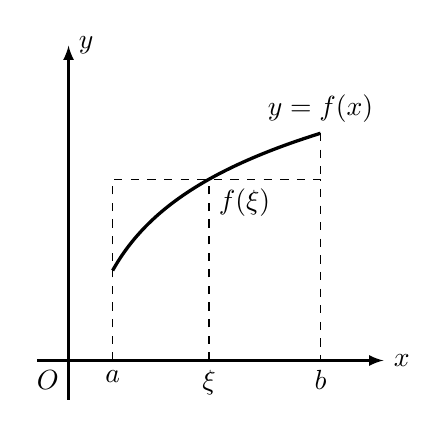
\begin{tikzpicture}[>=latex, xscale=.8]
\draw[->, thick](-.5,0)--(5,0)node[right]{$x$};
\draw[->, thick](0,-.5)--(0,4)node[right]{$y$};
\node at (0,0)[below left]{$O$};
\draw[domain=.7:4, very thick, samples=100]plot(\x, {ln(\x)+1.5})node[above]{$y=f(x)$};
\draw[dashed](.7,0)node[below]{$a$} rectangle (4,2.3);
\draw[dashed](2.23,0)node[below]{$\xi$}--(2.23,2.3)node[below right]{$f(\xi)$};
\draw[dashed](4,2.89)--(4,2.3);
\node at (4,0)[below]{$b$};

    \end{tikzpicture}
    \caption{}
    \end{minipage}
    \begin{minipage}[t]{0.48\textwidth}
    \centering
    \begin{tikzpicture}[>=latex, scale=.5]
  \draw[->, thick](-2,0)--(6,0)node[right]{$x$};
\draw[->, thick](0,-8.5)--(0,2)node[right]{$y$};
\node at (0,0)[below left]{$O$};
\draw[domain=-1:4, very thick, samples=100]plot(\x, {2*\x-\x*\x});
\fill[pattern=north east lines, domain=2:4, very thick, samples=100]plot(\x, {2*\x-\x*\x})--(4,0)node[above]{4}
--(2,0)node[above]{2};
\draw(1,0)node[below]{1}--(1,.2);
    \end{tikzpicture}
    \caption{}
    \end{minipage}
  \end{figure}

\begin{example}
求$\Int^4_2 (2x-x^2)\dd x$.
\end{example}


\begin{solution}
    根据本节的定积分计算法则得:
\[\begin{split}
    \Int^4_2 (2x-x^2)\dd x&=\Int^4_2 2x\dd x+\Int^4_2 (-x^2)\dd x\\
    &=2\Int^4_2 x\dd x-\Int^4_2 x^2\dd x
\end{split}\]
利用例3.4的计算结果,得
\[\Int^4_2 x\dd x=\frac{4^2-2^2}{2}=6,\qquad \Int^4_2 x^2\dd x=\frac{4^3-2^3}{3}=18\frac{2}{3}\]
因此
\[\Int^4_2 (2x-x^2)\dd x=2\x 6-18\frac{2}{3}=-6\frac{2}{3}\]
它的几何意义是图3.16中阴影区域的有号面积。
\end{solution}

\begin{example}
  设$f(x)=\begin{cases}
      x^2,& 0\le x\le 1\\
      1,& 1<x\le 2
  \end{cases}$,  求$f(x)$在$[0,2]$上的平均值.
\end{example}

\begin{solution}
由平均值定义,再利用性质1,有    
\[\begin{split}
    f(\xi)&=\frac{1}{b-a}\int^b_a f(x)\dd x=\frac{1}{2}\int^2_0 f(x)\dd x\\
    &=\frac{1}{2}\left[\int^1_0 f(x)\dd x+\int^2_1 f(x)\dd x\right]\\
    &=\frac{1}{2}\left[\int^1_0 x^2\dd x+\int^2_1 1\dd x\right]\\
    &=\frac{1}{2}\left[\frac{1}{3}+1\right]=\frac{2}{3}
\end{split}\]
\end{solution}

\begin{ex}
\begin{enumerate}
    \item 利用以前定积分的结果和定积分的性质,计算下列定积分:
\begin{enumerate}
    \item $\Int^3_{-1}(2x^2-4x)\dd x$
    \item 若$f(x)=\begin{cases}
        x,& 0\le x<1\\
        x-2,& 1\le x\le 2
    \end{cases}$,则$\Int^2_0 f(x)\dd x=?$
    \item 若$f(x)=\begin{cases}
        x,& 0\le x\le 1\\
        x-2,& 1< x\le 2
    \end{cases}$,则$\Int^2_0 f(x)\dd x=?$
\item 若$g(t)=2t^2+|t|-1,\; -1\le t\le 1$,则$\Int^1_{-1} g(t)\dd t=?$
\end{enumerate}

\item 将图中阴影部分的面积用定积分表示。
\item 设$\ell(t)=mt+b$, ($m,t$是常数),$t\in [c,d]$,

求证:$\Int^d_c (mt+b)\dd t=\frac{\ell(c)+\ell(d)}{2}(d-c)$
\item 证明:
\begin{enumerate}
    \item 若$0<x<10$,则$\frac{1}{1016}\le\frac{1}{x^3+16}\le \frac{1}{16}$
    \item $\frac{5}{508}\le \Int^{10}_0\frac{1}{x^3+16}\dd x\le \frac{5}{8}$
\end{enumerate}
\end{enumerate}
\end{ex}

\begin{figure}[htp]
    \centering
\begin{tikzpicture}[>=latex]
    
\begin{scope}[scale=.6]
\draw[->](-2,0)--(4,0)node[right]{$x$};
\draw[->](0,-3)--(0,7)node[right]{$y$};
\fill[domain=-1:3, samples=50, pattern=north east lines]plot(\x,{2*(\x-1)^2-2})--(3,0)--(-1,0)--(-1,6);
\draw[domain=-1:3, samples=50, very thick]plot(\x,{2*(\x-1)^2-2})node[above]{$y=2x^2-4x$};
\node at (0,0)[above right]{$O$};
\node at (-1,0)[below]{$-1$};
\node at (3,0)[below]{$3$};
\node at (-1,3)[left]{$x=-1$};
\node at (3,3)[right]{$x=3$};
\node at (1,-2)[below]{$(1,-2)$};
\node at (1,-3.8){(a)};
\end{scope}
\begin{scope}[xshift=5cm, yshift=-.8cm, scale=.9]
\draw[->](-1,0)--(4,0)node[right]{$x$};
\draw[->](0,-1)--(0,5.5)node[right]{$y$};
\node at (0,0)[below left]{$O$};
\draw[domain=0:2.2, samples=50, very thick]plot(\x,{\x^2})node[above]{$y=x^2$};
\draw[thick](0,0)--(3.5,3.5)node[right]{$y=x$};
\node at (1,0)[below]{$1$};
\node at (2,0)[below]{$2$};
\draw[dashed](0,1)node[left]{1}--(1,1)--(1,0);
\fill[domain=0:1, samples=50, pattern=north east lines]
plot(\x,{\x^2})--(2,2)--(2,0)--(0,0);
\node at (2,-1.5){(b)};
\end{scope}

\end{tikzpicture}
    \caption*{第2题}
\end{figure}



\subsection*{习题3.2}
\begin{enumerate}
    \item 计算下列定积分:
\begin{multicols}{3}
\begin{enumerate}
    \item $\Int^1_4 |x|\dd x$
    \item $\Int^2_4 |x|\dd x$
    \item $\Int^4_1 |x|\dd x$
\end{enumerate}
\end{multicols}
\item 求$\Int^b_a |x|\dd x$.

提示:分$a<b<0$, $a<0<b$, $0<a<b$三种情况讨论。
\item 证明:
\begin{enumerate}
    \item 若$\frac{\pi}{4}\le x\le\frac{\pi}{2}$,则$\frac{2}{\pi}\le \frac{\sin x}{x}\le \frac{2\sqrt{2}}{\pi}$
    \item $\frac{1}{2}\le \Int^{\tfrac{\pi}{2}}_{\tfrac{\pi}{4}}\frac{\sin x}{x}\dd x\le \frac{\sqrt{2}}{2}$
\end{enumerate}
\item 已知作用在作直线运动的质点上的力是$F=s^2+1$, 试求从距离1到10之间所作的功.
\item 求$y=\begin{cases}
    A\sin\frac{2\pi t}{T}, & 0\le t\le \frac{T}{2}\\
    0,& \frac{T}{2}\le t\le T
\end{cases}$ 在$[0,T]$上的平均值。
\end{enumerate}